\subsection*{Lösungen zu Kapitel~\ref{kapitel:Potenzgeraden}: \emph{Potenzgeraden}}
\begin{proof}[Lösung zu Aufgabe~\ref{aufgabe:VonAOPSGeklaut}]
	Wenn $PQRS$ ein Sehnenviereck ist, dann schneiden sich $PQ$, $RS$ und $XY$ in einem Punkt $Z$, denn bei diesen Geraden handelt es sich um die paarweisen Potenzgeraden der Kreise $\omega_1$, $\omega_2$ und $\odot PQRS$.
	
	Seien nun $O_1$, $O_2$ und $O$ die Mittelpunkte der Kreise $\omega_1$, $\omega_2$ und $\odot PQRS$. Wenn sich zwei Kreise schneiden, dann steht die Verbindungsgerade ihrer Mittelpunkte stets senkrecht auf der Verbindungsgeraden der beiden Schnittpunkte. Insbesondere steht $OO_1$ senkrecht auf der Geraden $RS$. Weil $RS$ nach Annahme durch $O_2$ verläuft, muss $RS$ also die Höhe durch $O_2$ im Dreieck $OO_1O_2$ sein. Analog ist $PQ$ die Höhe durch $O_1$. Ihr Schnittpunkt~$Z$ ist somit der Höhenschnittpunkt von $OO_1O_2$. Folglich muss $OZ$ die Höhe durch $O$ sein. Also steht $OZ$ senkrecht auf $O_1O_2$. Die Gerade $XY$ verläuft aber ebenfalls durch~$Z$ und steht senkrecht auf $O_1O_2$. Folglich müssen die Geraden $OZ$ und $XY$ identisch sein, sodass $O$ auf $XY$ liegt.
\end{proof}

\begin{figure}[ht]
	\centering
	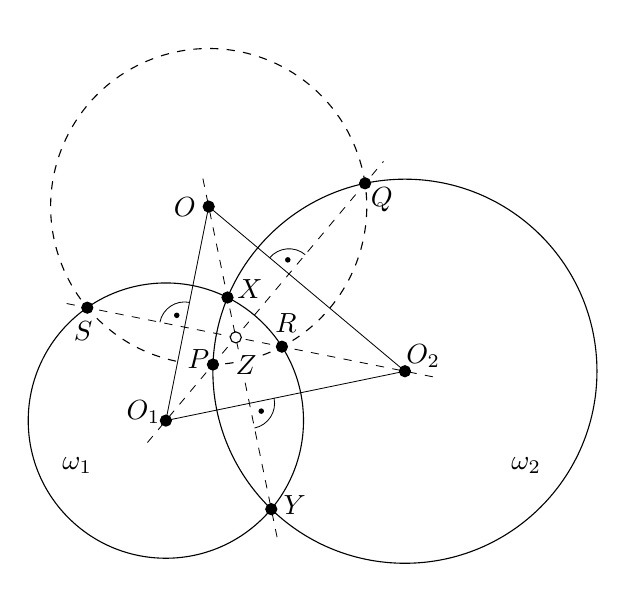
\begin{tikzpicture}
		\draw (-2.675,0.566) coordinate (O1) circle (1.748);
		\draw (0.361,1.193) coordinate (O2) circle (2.439);
		\coordinate (O) at (-2.131,3.284);
		\draw[dashed,shift={(O)}]  (-70:2.007) arc (-70:260:2.007);
		\draw[dashed,shift={(O)}]  (270:2.007) arc (270:280:2.007);
		\coordinate (P) at (-2.077,1.278);
		\coordinate (Q) at (-0.145,3.579);
		\coordinate (R) at (-1.201,1.505);
		\coordinate (S) at (-3.673,2);
		\coordinate (X) at (-1.892,2.129);
		\coordinate (Y) at (-1.336,-0.559);
		\coordinate (Z) at (-1.787,1.623);
		\draw[dashed,line width=0.3, shorten <=-2.4ex,shorten >=3.5ex] (Y) to (Z);
		\draw[dashed,line width=0.3, shorten <=-2.4ex,shorten >=-1.5ex] (O) to (Z);
		\draw[dashed,line width=0.3, shorten <=-2.4ex,shorten >=-2.4ex] (O1) to (Q);
		\draw[dashed,line width=0.3, shorten <=-2.4ex,shorten >=-2.4ex] (O2) to (S);
		\draw[line width=0.3,shift={(-2.437,1.753)}] (78.685:0.32cm) arc (78.685:168.685:0.32cm);
		\fill[shift={(-2.437,1.753)}] (123.685:0.18cm) circle (1pt);
		\draw[line width=0.3,shift={(-1.111,2.428)}] (49.991:0.32cm) arc (49.991:139.991:0.32cm);
		\fill[shift={(-1.111,2.428)}] (94.991:0.18cm) circle (1pt);
		\draw[line width=0.3,shift={(-1.614,0.785)}] (281.679:0.32cm) arc (281.679:371.679:0.32cm);
		\fill[shift={(-1.614,0.785)}] (326.679:0.18cm) circle (1pt);
		\draw[line width=0.3] (O1) to (O2) to (O) to cycle;
		\draw[fill=black] (O1) circle (2pt) node[shift={(160:2ex)}] {$O_1$};
		\draw[fill=black] (O2) circle (2pt) node[shift={(40:2ex)}] {$O_2$};
		\draw[fill=black] (O) circle (2pt) node[shift={(180:2ex)}] {$O$};
		\draw[fill=black] (P) circle (2pt) node[shift={(160:1.3ex)}] {$P$};
		\draw[fill=black] (Q) circle (2pt) node[shift={(315:2ex)}] {$Q$};
		\draw[fill=black] (R) circle (2pt) node[shift={(80:2ex)}] {$R$};
		\draw[fill=black] (S) circle (2pt) node[shift={(260:2ex)}] {$S$};
		\draw[fill=black] (X) circle (2pt) node[shift={(20:2ex)}] {$X$};
		\draw[fill=black] (Y) circle (2pt) node[shift={(10:2ex)}] {$Y$};
		\draw[fill=white] (Z) circle (2pt) node[shift={(290:2.5ex)}] {$Z$};
		\node at (-3.8,0) {$\omega_1$};
		\node at (1.9,0) {$\omega_2$};
	\end{tikzpicture}
\end{figure}
	
\begin{proof}[Lösung zu Aufgabe~\ref{aufgabe:IMO1995_1}]
	Unser Ziel ist zu zeigen, dass $ADNM$ ein Sehnenviereck ist, denn dann handelt es sich bei $AM$, $DN$ und $XY$ um die paarweisen Potenzgeraden der Kreise $\omega_1$,~$\omega_2$ und~$ADNM$, welche sich in einem Punkt schneiden.
	
	\begin{figure}[ht]
		\centering
		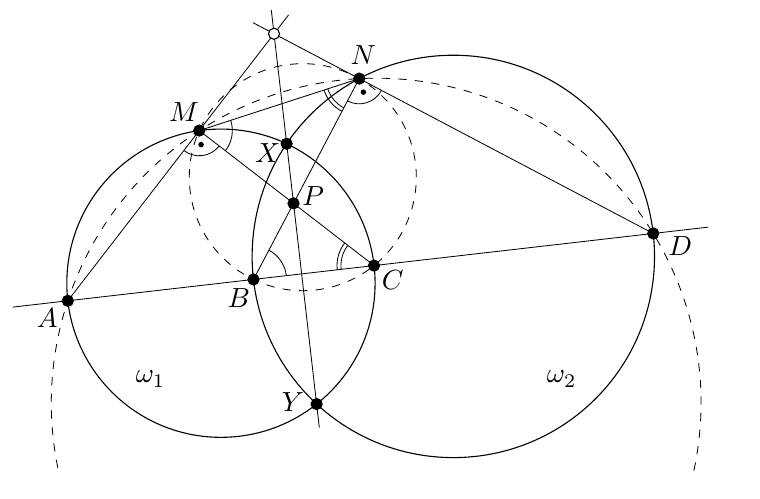
\begin{tikzpicture}[x=0.9cm,y=0.9cm]
			\draw (-1.007,2.103) circle (2.175);
			\draw (2.272,2.481) circle (2.839);
			\draw[line width=0.3,dashed] (0.148,3.599) circle (1.602);
			\draw[line width=0.3,dashed,shift={(1.183,0.412)}]  (-12:4.584) arc (-12:192:4.584);
			\coordinate (A) at (-3.168,1.855);
			\coordinate (B) at (-0.548,2.156);
			\coordinate (C) at (1.153,2.352);
			\coordinate (D) at (5.093,2.805);
			\coordinate (M) at (-1.313,4.257);
			\coordinate (N) at (0.944,4.99);
			\coordinate (P) at (0.017,3.23);
			\coordinate (X) at (-0.08,4.071);
			\coordinate (Y) at (0.343,0.398);
			\coordinate (Z) at (-0.258,5.623);
			\draw[line width=0.3,shift={(M)}] (-37.679:0.42cm) arc (-37.679:17.987:0.42cm);
			\draw[line width=0.3,shift={(M)}] (-127.679:0.32cm) arc (-127.679:-37.679:0.32cm);
			\fill[shift={(M)}] (-82.679:0.18cm) circle (1pt);
			\draw[line width=0.3,shift={(B)}] (6.561:0.42cm) arc (6.561:62.257:0.42cm);
			\draw[line width=0.3,shift={(N)}] (197.988:0.47cm) arc (197.988:242.228:0.47cm);
			\draw[line width=0.3,shift={(N)}] (197.988:0.42cm) arc (197.988:242.228:0.42cm);
			\draw[line width=0.3,shift={(N)}] (242.228:0.32cm) arc (242.228:332.228:0.32cm);
			\fill[shift={(N)}] (287.228:0.18cm) circle (1pt);
			\draw[line width=0.3,shift={(C)}] (142.321:0.42cm) arc (142.321:186.561:0.42cm);
			\draw[line width=0.3,shift={(C)}] (142.321:0.47cm) arc (142.321:186.561:0.47cm);
			\draw[line width=0.3,shorten <=-2em,shorten >=-2em] (A) to (D);
			\draw[line width=0.3,shorten >=-2ex] (A) to (Z);
			\draw[line width=0.3,shorten >=-2ex] (D) to (Z);
			\draw[line width=0.3,shorten <=-2ex,shorten >=-2ex] (Y) to (Z);
			\draw[line width=0.3] (M) to (N);
			\draw[line width=0.3] (B) to (N);
			\draw[line width=0.3] (C) to (M);
			\draw[fill=black] (A) circle (2pt) node[shift={(220:2.25ex)}] {$A$};
			\draw[fill=black] (B) circle (2pt) node[shift={(232:2ex)}] {$B$};
			\draw[fill=black] (C) circle (2pt) node[shift={(-38:2ex)}] {$C$};
			\draw[fill=black] (D) circle (2pt) node[shift={(-25:2.5ex)}] {$D$};
			\draw[fill=black] (M) circle (2pt) node[shift={(130:2ex)}] {$M$};
			\draw[fill=black] (N) circle (2pt) node[shift={(80:2ex)}] {$N$};
			\draw[fill=black] (P) circle (2pt) node[shift={(20:1.75ex)}] {$P$};
			\draw[fill=black] (X) circle (2pt) node[shift={(205:1.75ex)}] {$X$};
			\draw[fill=black] (Y) circle (2pt) node[shift={(175:2ex)}] {$Y$};
			\draw[fill=white] (Z) circle (2pt);
			\node at (-2,0.75) {$\omega_1$};
			\node at (3.8,0.75) {$\omega_2$};
		\end{tikzpicture}
	\end{figure}
	
	Nach dem Sehnensatz in den Kreisen $\omega_1$ und~$\omega_2$ gilt $\abs*{CP}\cdot \abs*{MP}=\abs*{XP}\cdot \abs*{YP}=\abs*{BP}\cdot \abs{NP}$. Nach der Umkehrung des Sehnensatzes ist $BCNM$ also ein Sehnenviereck. Nach dem Satz des Thales gilt $\winkel AMC=90^\circ=\winkel BND$. Also ist $\winkel CAM=180^\circ-\winkel AMC-\winkel MCA=90^\circ-\winkel MCA$. Nach dem Peripheriewinkelsatz im Sehnenviereck $BCNM$ gilt aber auch $\winkel MCA=\winkel NMA$. Es folgt
	\begin{equation*}
		\winkel DAM+\winkel MND=\winkel CAM+\winkel MNB+\winkel BND=\parens*{90^\circ-\winkel MCA}+\winkel MCA+90^\circ=180^\circ\,.
	\end{equation*}
	Folglich muss $ADNM$ ein Sehnenviereck sein und wir sind fertig.
\end{proof}
\begin{proof}[Lösung zu Aufgabe~\ref{aufgabe:VAIMO2012_2}]
	Sei $I$ der Schnittpunkt der Winkelhalbierenden von $\winkel BMN$ mit der Winkelhalbierenden von$ \winkel ACB$. Dann ist $I$ der Inkreismittelpunkt des Dreiecks $AMC$. Wir werden zeigen, dass $ABMI$ und $CIMN$ Sehnenvierecke sind. Wenn wir das zeigen können, sind wir fertig. Denn dann folgt, dass $AB$, $CP$ und die Winkelhalbierende von $\winkel BMN$ die paarweisen Potenzgeraden der Kreise $\odot ABC$, $\odot CIMN$ und $\odot ABMI$ sind. Also schneiden sie sich in einem Punkt. Folglich liegt der Schnittpunkt~$Q$ von $AB$ und $CP$ auf der Winkelhalbierenden von $\winkel BMN$, wie behauptet.
	
	\begin{figure}[ht]
		\centering
		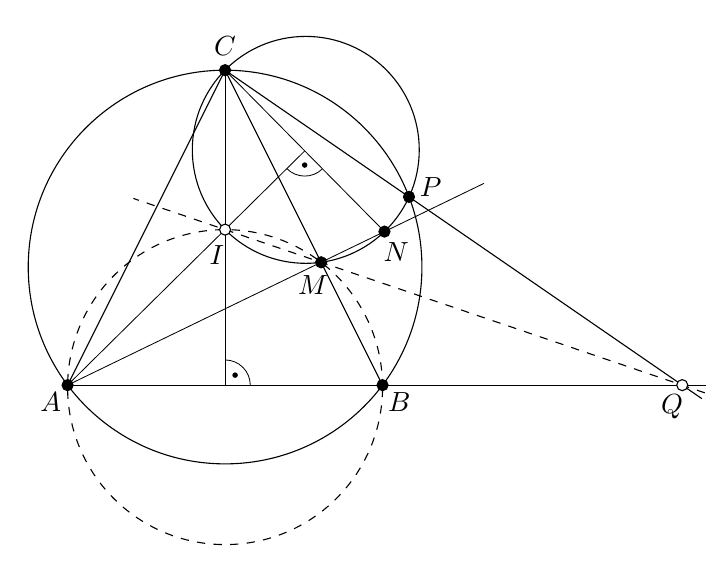
\begin{tikzpicture}
			\draw (0,1.5) circle (2.5);
			\draw[,dashed] (0,-0.025) circle (2);
			\draw (1.025,2.988) circle (1.441);
			\coordinate (A) at (-2,0);
			\coordinate (B) at (2,0);
			\coordinate (C) at (0,4);
			\coordinate (I) at (0,1.975);
			\coordinate (M) at (1.22,1.56);
			\coordinate (N) at (2.024,1.95);
			\coordinate (P) at (2.336,2.391);
			\coordinate (Q) at (5.806,0);
			\coordinate (midCN) at (1.012,2.975);
			\draw[line width=0.3,shift={(0,0)}] (0:0.32cm) arc (0:90:0.32cm);
			\fill[shift={((0,0))}] (45:0.18cm) circle (1pt);
			\draw[line width=0.3,shift={(midCN)}] (224.646:0.32cm) arc (224.646:314.646:0.32cm);
			\fill[shift={(midCN)}] (269.646:0.18cm) circle (1pt);
			\draw (A) to (C) to (B);
			\draw[line width=0.3] (C) to (0,0);
			\draw[line width=0.3] (A) to (midCN);
			\draw[shorten >=-2ex] (A) to (Q);
			\draw[shorten >=-2ex] (C) to (Q);
			\draw[dashed,shorten <=-2ex,shorten >=-3.5em] (Q) to (I);
			\draw[line width=0.3,shorten >=-4em] (A) to (N);
			\draw[line width=0.3] (C) to (N);
			\draw[fill=black] (A) circle (2pt) node[shift={(225:2ex)}] {$A$};
			\draw[fill=black] (B) circle (2pt) node[shift={(315:2ex)}] {$B$};
			\draw[fill=black] (C) circle (2pt) node[shift={(90:2ex)}] {$C$};
			\draw[fill=white] (I) circle (2pt) node[shift={(252:2.25ex)}] {$I$};
			\draw[fill=black] (M) circle (2pt) node[shift={(250:2ex)}] {$M$};
			\draw[fill=black] (N) circle (2pt) node[shift={(300:2ex)}] {$N$};
			\draw[fill=black] (P) circle (2pt) node[shift={(25:2ex)}] {$P$};
			\draw[fill=white] (Q) circle (2pt) node[shift={(245:2ex)}] {$Q$};
		\end{tikzpicture}
	\end{figure}
	
	Gemäß dem Südpolsatz (bzw.\ in diesem Fall dem \enquote{Nordpolsatz}) schneiden sich die Mittelsenkrechte von $\overline{CN}$ und die Außenwinkelhalbierende von $\winkel NMC$ auf dem Umkreis $\odot CMN$. 
	Nach Voraussetzung gilt $\abs*{AC}=\abs*{AN}$, also ist die Mittelsenkrechte von $\overline{CN}$ auch die Winkelhalbierende von $\winkel MAC$. Ferner ist die Außenwinkelhalbierende von $\winkel NMC$ auch die Winkelhalbierende von $\winkel CMA$. Somit ist der betrachtete Schnittpunkt genau der Inkreismittelpunkt von $AMC$. Damit haben wir gezeigt, dass $I$ auf dem Umkreis $\odot CMN$ liegt, sodass $CIMN$ ein Sehnenviereck ist.
	
	Nach dem \enquote{Nordpolsatz} schneiden sich außerdem die Mittelsenkrechte von $\overline{AB}$ und die Außenwinkelhalbierende von $\winkel AMB$ auf dem Umkreis $\odot ABM$. Wegen $\abs*{AC}=\abs*{BC}$ ist die Mittelsenkrechte von $\overline{AB}$ gleichzeitig die Winkelhalbierende von $\winkel ACB$. Ferner ist die Außenwinkelhalbierende von $\winkel AMB$ auch die Winkelhalbierende von $\winkel CMA$. Somit ist~$I$ wieder der betrachtete Schnittpunkt. Damit haben wir gezeigt, dass $I$ auf dem Umkreis $\odot ABM$ liegt, sodass $ABMI$ ein Sehnenviereck ist.
\end{proof}
\begin{proof}[Lösung zu Aufgabe~\ref{aufgabe:Ceva+Brianchon}]
	Indem wir den Satz von Brianchon auf das entartete Tangentensechseck $AWBXCD$ anwenden, erhalten wir, dass sich dessen Hauptdiagonalen $AX$, $CW$ und $BD$ in einem Punkt $Q$ schneiden. Aus dem Satz von Ceva folgt sodann
	\begin{equation*}
		\frac{\abs*{AP}}{\abs*{CP}}\cdot \frac{\abs*{CX}}{\abs*{BX}}\cdot \frac{\abs*{BW}}{\abs*{AW}}=1\,.
	\end{equation*}
	Nun gilt aber auch $\abs*{BW}=\abs*{BX}$, denn bei den Strecken $\overline{BW}$ und $\overline{BX}$ handelt es sich um die Tangentenabschnitte von $B$ an den Inkreis von $ABCD$. Durch Einsetzen in die obige Gleichung erhalten wir
	\begin{equation*}
		\frac{\abs*{AP}}{\abs*{CP}}\cdot \frac{\abs*{CX}}{\abs*{AW}}=1\,,\quad\text{also}\quad \frac{\abs*{AP}}{\abs*{CP}}= \frac{\abs*{AW}}{\abs*{CX}}\,.
	\end{equation*}
	Damit ist die erste der gewünschten Verhältnisgleichungen gezeigt. Wieder aufgrund gleichlanger Tangentenabschnitte gilt $\abs*{AZ}=\abs*{AW}$ und $\abs*{CY}=\abs*{CX}$. Daraus folgt sofort die zweite Verhältnisgleichung.
\end{proof}
\begin{figure}[ht]
	\centering
	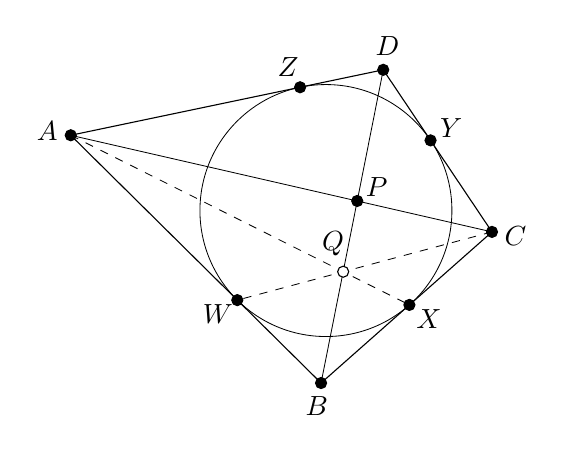
\begin{tikzpicture}[x=0.8cm,y=0.8cm]
		\draw[line width=0.3] (0,0) circle (2);
		\coordinate (A) at (-4.051,1.195);
		\coordinate (B) at (-0.077,-2.738);
		\coordinate (C) at (2.636,-0.339);
		\coordinate (D) at (0.91,2.234);
		\coordinate (P) at (0.497,0.152);
		\coordinate (Q) at (0.274,-0.971);
		\coordinate (W) at (-1.407,-1.422);
		\coordinate (X) at (1.325,-1.498);
		\coordinate (Y) at (1.661,1.114);
		\coordinate (Z) at (-0.41,1.957);
		\draw (A) to (B) to (C) to (D) to cycle;
		\draw[line width=0.3] (A) to (C);
		\draw[line width=0.3] (B) to (D);
		\draw[line width=0.3,dashed] (A) to (X);
		\draw[line width=0.3,dashed] (C) to (W);
		\draw[fill=black] (A) circle (2pt) node[shift={(170:2ex)}] {$A$};
		\draw[fill=black] (B) circle (2pt) node[shift={(260:2ex)}] {$B$};
		\draw[fill=black] (C) circle (2pt) node[shift={(-10:2ex)}] {$C$};
		\draw[fill=black] (D) circle (2pt) node[shift={(80:2ex)}] {$D$};
		\draw[fill=black] (P) circle (2pt) node[shift={(35:2ex)}] {$P$};
		\draw[fill=white] (Q) circle (2pt) node[shift={(110:2.5ex)}] {$Q$};
		\draw[fill=black] (W) circle (2pt) node[shift={(215:2ex)}] {$W$};
		\draw[fill=black] (X) circle (2pt) node[shift={(-35:2ex)}] {$X$};
		\draw[fill=black] (Y) circle (2pt) node[shift={(30:2ex)}] {$Y$};
		\draw[fill=black] (Z) circle (2pt) node[shift={(120:2ex)}] {$Z$};
	\end{tikzpicture}
\end{figure}